\documentclass[12pt, a4paper]{article}
\usepackage{amsmath}
\usepackage{amsfonts}
\usepackage{amsthm}
\usepackage{mathtools}
\newtheorem{theorem}{Theorem}[section]
\newtheorem{definition}{Definition}[section]
\numberwithin{equation}{section}
\usepackage{pgfplots}
\pgfplotsset{width=10cm,compat=1.9}
\graphicspath{ {img/} }
\DeclareGraphicsExtensions{.png,.jpg}

\title{Support Vector Machines}
\author{Kristian Wichmann}

\begin{document}
\maketitle

\section{Overview}
At its heart, a \textit{support vector machine} (SVM) is a binary classifaction algorithm. The basic version creates a linear decision boundary, but using a strategy known as the \textit{kernel trick}, we can make SVM's produce non-linear decision boundaries.

\section{Linearly separable data}
Initially, we assume that the data can be perfectly classified by a linear decision boundary - a hyperplane in configuration space such that all positives are on one side and all negatives on the other side. Generally, this can be done in many ways. So we will specifically search for the one which maximizes the perpendicular distance to the closest data points. Such closest point are known as \textit{support vectors}. See figure \ref{fig:svm_linear}.

\begin{figure}
\centering
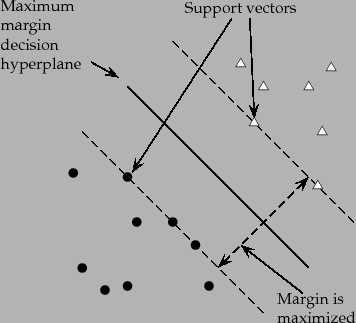
\includegraphics[scale=0.5]{svm1}
\caption{We're searching for the widest possible separation "road".}
\label{fig:svm_linear}
\end{figure}

\subsection{Classifying a new data point}
If we have a new data point $\vec{u}$, we might ask whether or not our algorithm classifies $\vec{u}$ as a positive or a negative.

The separation boundary is a hyperplane. Let $\vec{w}$ be a normal vector to this hyperplane\footnote{The chosen vector is sometimes referred to as the \textit{weight vector}.}. We want to know how far in the direction of $\vec{w}$ our new data point $\vec{u}$ goes. In other words, we want to know the projection of $\vec{u}$ on $\vec{w}$:
\begin{equation}
\vec{u}_{\vec{w}}=\frac{\vec{u}\cdot\vec{w}}{|\vec{w}|^2}\vec{w}
\end{equation}
So the signed distance from the origin to $\vec{u}$ is proportional to the inner product $\vec{u}\cdot\vec{w}$. Using more compact notation, this can also be written $u^T w=w^t u$. Since the decision boundary is perpendicular to $w$, this inner product will have the same value for all points on it. We will call this value $-b$. Thus, the expression $w^T u+b$ will be exactly zero on the boundary, and its sign will otherwise decide which side the new data point is on. Hence, we may write the classifier as a function $f$:
\begin{equation}
f(u)=\textrm{sign}(w^T u+b)
\end{equation}
Here, positives are identifies as $+1$ and negatives as $-1$\footnote{If these happen to be switched around, $-w$ will do the trick instead}.

\end{document}